\section{Experiments}
One primary experiment was run to test the effectiveness of the mass neural network, the adaptive controller, and the Kalman filter.
This was the task proposed in the introduction, consisting of three phases.
Each of these phases provided different data to be collected and measured to see how well each method performed.
In addition, the loss metrics of the mass neural network during training will be plotted and discussed.

\subsection*{Controls Experiment}
Both the adaptive control and the mass matrix neural network control were tested against each other in the three different phases.
These phases consisted of the initial trajectory towards the target object, moving the object of unknown mass to the goal state, and finally returning to the original position the arm started in.
Both of these methods were compared to a baseline of a standard PD trajectory tracking controller as well, to serve as a baseline for performance.
The metric for these experiments was the error in tracked trajectory for both joint configurations and velocities under control.

\subsubsection*{Mass Experiment}
The adaptive control was also tested multiple times in the second phase (moving the object of unknown mass) where the mass was varied.
The performance under differing weights was of particular interest.
The metric for this experiment was the error in tracked trajectory for the three joint configurations and velocities during the control.

\subsection*{Kalman Filter Experiment}
To measure the effectiveness of the Kalman filter, both the stationary and moving filter results were examined.
The error in actual position (known due to simulation) versus predicted position was used as the metric.
If effectively implemented, the error in predicted position should begin to converge towards the actual position as more samples are acquired and the confidence of the filter increases.

The experiments will use white noise samples from the Gaussian distribution $n\sim \mathcal{N}(0,0.1)$.
This variance provides enough noise to show the filter working effectively, but not so much that it cannot provide accurate estimates within the short time span of the trajectory.

\subsection*{Control Models}
To validate our control models, it is important to evaluate the error dynamics associated with the controllers. To do this, we begin with the comparison of the error convergence between the Adaptive Control model and the classical PD Control model. This comparison was made with a fixed, known weight, as well as no noise in the joint values.
\begin{figure}[H]
	\centering
	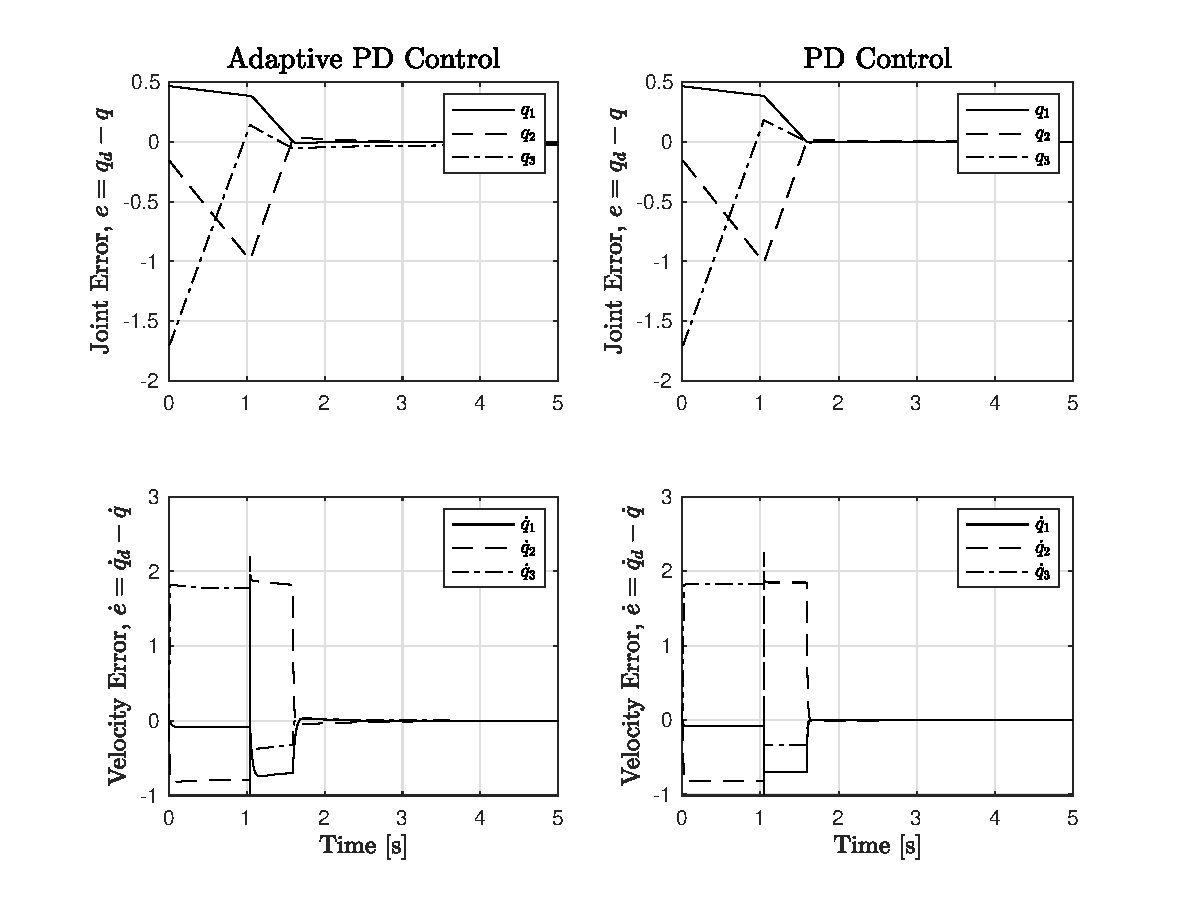
\includegraphics[width=0.7\textwidth]{figures/adpdErr.eps}
	\caption{Convergence of controller error dynamics}
	\label{fig:adpderr}
\end{figure}
As shown in Fig. \ref{fig:adpderr}, both controllers converge to the steady state value of zero in approximately the same time. One benefit to adaptive control however, is that as the mass changes (i.e. an object is picked up), the adaptation law accounts for the change in mass. With PD Control, there is no way to account for this mass addition and an increase in error is introduced.\\

We then evaluate each controller by it's ability to follow the desired trajectory provided by the $RRT^{*}$ path planning algorithm.
\begin{figure}[H]
	\centering
	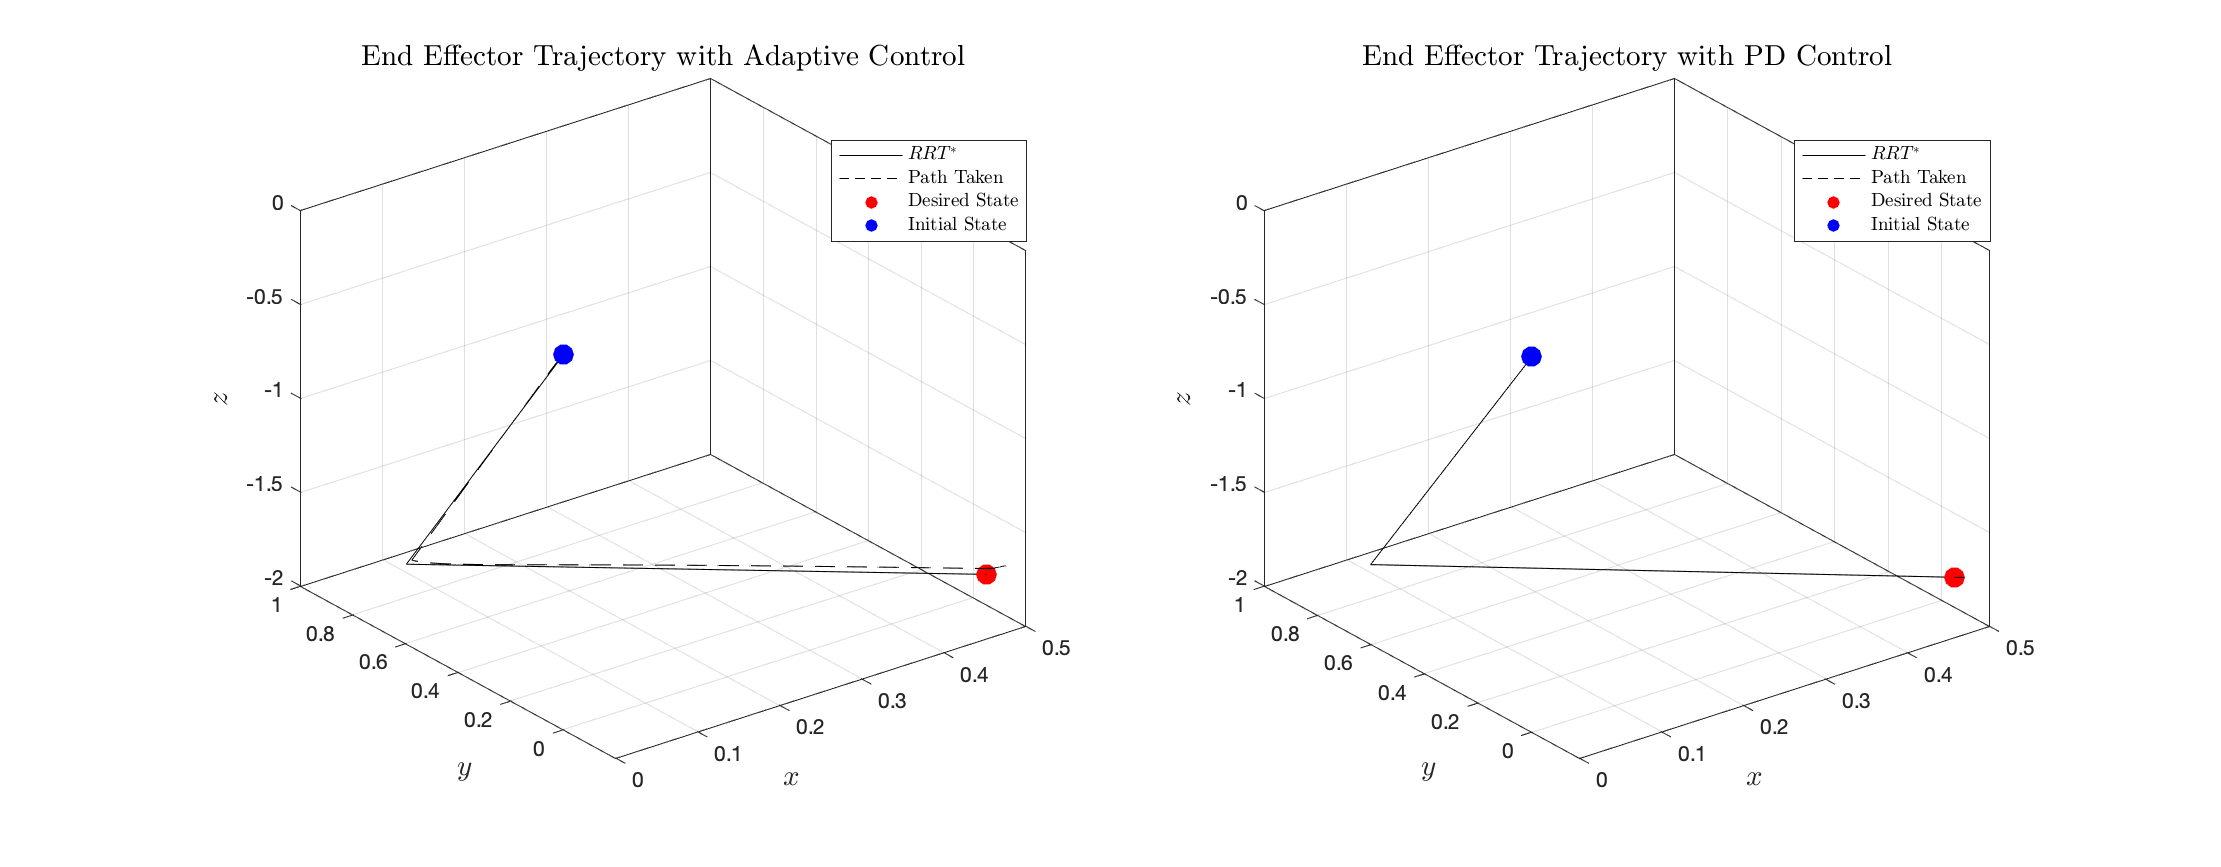
\includegraphics[width=0.9\textwidth]{figures/eeTraj.eps}
	\caption{Desired end-effector trajectory vs actual}
	\label{fig:eetraj}
\end{figure}
We can see from Fig. \ref{fig:eetraj} that in this case, the PD Controller maintains the desired trajectory more tightly than the Adaptive Control model. However, the error between the two control models is of an insignificant degree, thus the adaptive control model is chosen for the simulation.

